\documentclass[14pt]{extarticle}
\usepackage{fontspec}
\usepackage{polyglossia}
\usepackage{amsmath}
\usepackage{amssymb}
\usepackage{xcolor}
\usepackage{fancyhdr}
\usepackage{graphicx}
\usepackage{listings}
\usepackage[most]{tcolorbox}
% \usepackage{setspace}
\usepackage{pifont}
\usepackage{enumitem}
\usepackage{titlesec}
\usepackage[bottom]{footmisc}
\usepackage{titling}
\usepackage{minted}
\usepackage{etoolbox}
\usepackage{array}
\usepackage{extsizes}
\usepackage{float}
\usepackage{booktabs}
\usepackage{hyperref}
\usepackage[onehalfspacing]{setspace}
\usepackage[a4paper, top=2.7cm, bottom=2.7cm, left=2.5cm, right=2.5cm, headheight=1.5cm, headsep=0.5cm]{geometry}
\usepackage{tikz}

\usetikzlibrary{automata, positioning, arrows.meta, arrows}

\newfontfamily\emoji{Segoe UI Emoji}

\pagestyle{fancy}

\setmainlanguage[numerals=western]{arabic}
\setotherlanguage{english}
% \newfontfamily\arabicfont[Script=Arabic]{Amiri}
\newfontfamily\arabicfont[Script=Arabic]{Calibri}
\newfontfamily\arabicfonttt[Script=Arabic]{Courier New}

\lstset{
  language=[Sharp]C,
  numbers=left,
  stepnumber=1,
  numbersep=8pt,
  frame=single,
  basicstyle=\ttfamily\small,
  keywordstyle=\color{blue},
  stringstyle=\color{red},
  commentstyle=\color{green!50!black}
}

\newif\ifdetailed
\ifdefined\setdetailed
  \setdetailed
\fi

\newif\ifwithsols
\ifdefined\setwithsols
  \setwithsols
\fi

% unified tcolorboxes for articles
\tcbset{colback=white, colframe=black, fonttitle=\bfseries, boxrule=0.8pt}
\newtcolorbox{boxDef}[1][]{colback=blue!5!white,colframe=blue!75!black,
  title={{\emoji📘} تعريف\ifx\\#1\\\else ~#1\fi :}}
\newtcolorbox{boxExercise}[1][]{colback=cyan!5!white,colframe=cyan!70!black,
  title={{\emoji🧩} تمرين\ifx\\#1\\\else ~#1\fi :}}
\newtcolorbox{boxExample}[1][]{colback=yellow!5!white,colframe=orange!90!black,
  title={{\emoji📝} مثال\ifx\\#1\\\else ~#1\fi :}}
\newtcolorbox{boxNote}[1][]{colback=gray!10!white,colframe=black,
  title={{\emoji✨} ملاحظة\ifx\\#1\\\else ~#1\fi :}}
\newtcolorbox{boxAttention}[1][]{colback=magenta!10!white,colframe=magenta!80!black,
  title={{\emoji🔔} تنبيه\ifx\\#1\\\else ~#1\fi :}}
\newtcolorbox{boxWarning}[1][]{colback=red!5!white,colframe=red!75!black,
  title={{\emoji⚡} ملاحظة هامة\ifx\\#1\\\else ~#1\fi :}}
\newtcolorbox{boxSolution}[1][]{colback=green!5!white,colframe=green!60!black,
  title={{\emoji✅} حل\ifx\\#1\\\else ~#1\fi :}}
\newtcolorbox{boxSymbol}[1][]{colback=purple!5!white,colframe=purple!70!black,
  title={{\emoji🔣} رمز\ifx\\#1\\\else ~#1\fi :}}
\newtcolorbox{boxHint}[1][]{colback=teal!5!white,colframe=teal!60!black,
  title={{\emoji💡} تلميح\ifx\\#1\\\else ~#1\fi :}}


\tcbset{simplecode/.style={ colback=gray!5, colframe=black!50, boxrule=0.4pt, arc=2pt, left=4pt,right=4pt,top=4pt,bottom=4pt}}
\newenvironment{boxCode}{\begin{tcolorbox}[simplecode]}{\end{tcolorbox}}

\newcolumntype{C}[1]{>{\centering\arraybackslash}p{#1}}

% redefine spaces after titles
\makeatletter
\renewcommand{\@maketitle}{%
  \begin{center}
    {\huge \bfseries \@title \par}%
    \vskip 0.2em % space between title and author
    {\large \@author \par}%
    % \vskip 0.2em % space between author and date
    % {\normalsize \@date \par}%
  \end{center}
}
\makeatother

\fancyhf{} % clear default
\fancypagestyle{plain}{
  \fancyhf{}
  \fancyhead[L]{مدرسة التسامح الشاملة}
  % \fancyhead[L]{
\includegraphics[height=1cm]{../../../images/logoTasamoh.png}}
  \fancyhead[R]{الأستاذ محمود اغبارية}
  \fancyfoot[C]{\thepage}
}

\fancyhead[L]{مدرسة التسامح الشاملة}
\fancyhead[R]{الأستاذ محمود اغبارية}
\fancyfoot[C]{\thepage}
% \date{\today}

\setcounter{tocdepth}{3} % only section subsection and subsubsection in TOC

\newcommand{\importpdfpage}[2]{%
    \thispagestyle{empty}
    \newgeometry{left=0cm,right=0cm,top=0cm,bottom=0cm}
    \includegraphics[page=#2,width=0.95\paperwidth,height=0.95\paperheight,keepaspectratio]{#1}
    \restoregeometry
}

\newcommand{\insertFullImg}[1]{%
    \noindent
    \makebox[\textwidth][c]{
        \includegraphics[width=0.9\paperwidth,keepaspectratio]{#1}%
    }%
}%

% ----------------------


% \begin{document}

% \maketitle

% % \clearpage  % start TOC on a new page
% % \renewcommand{\contentsname}{جدول المحتويات}
% % \tableofcontents
% % \clearpage

% \part*{part 1} % the * prevents numbering
% \section*{مقدمة}
% \subsection*{مثال رياضي}
% \subsubsection*{مثال فرعي}
% \paragraph*{ paragraph 1}
% \subparagraph*{sub paragraph 1}

% \ifdetailed
% \begin{english}
% \begin{minted}{csharp}
% // C# Example
% \end{minted}
% \end{english}
% \fi

% OLD WAY
% \ifdetailed
% \begin{english}
% \begin{lstlisting}
% // C# Example
% \end{lstlisting}
% \end{english}
% \fi

% % 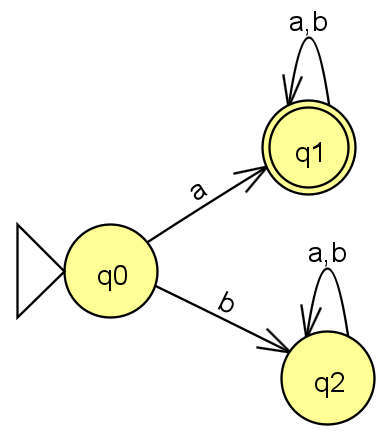
\includegraphics[width=0.2\textwidth]{../../../images/DFAs/ex1_q1.png}



% \vspace{3cm}
% \begin{flushleft}
% أرجو لكم وقتًا ممتعًا.

% الأستاذ محمود اغبارية.
% \end{flushleft}


% \end{document}


\title{ملخّص الدرس: الفئات والكائنات المتقدّمة في \textenglish{C\#}}

\begin{document}

\maketitle
\thispagestyle{fancy}

%=============================================================
\section{مصفوفة من الكائنات}
%=============================================================

تمامًا كما نُعرِّف مصفوفة من الأعداد أو النصوص، يمكننا تعريف مصفوفة من الكائنات.

\begin{boxExample}
\begin{english}
\begin{minted}{csharp}
// In Main
Book[] library = new Book[3];
library[0] = new Book("Algebra",   "Teacher", 2020, 100.0);
library[1] = new Book("Geometry",  "Teacher", 2022, 150.0);
library[2] = new Book("Physics",   "Teacher", 2021, 120.0);
\end{minted}
\end{english}
\end{boxExample}

\begin{itemize}[itemsep=1pt]
    \item السطر الأول يُنشئ المصفوفة فقط — خاناتها تحتوي \textenglish{null} في البداية.
    \item كل عنصر يحتاج \textenglish{new Book(...)} منفصلًا لإنشاء الكائن الفعلي.
\end{itemize}

للمرور على المصفوفة نستخدم حلقة \textenglish{for} عادية:

\begin{boxExample}
\begin{english}
\begin{minted}{csharp}
// In Main
for (int i = 0; i < library.Length; i++)
    library[i].Print();
\end{minted}
\end{english}
\end{boxExample}

يمكن أيضًا استخدام حلقة \textenglish{foreach}:

\begin{boxExample}
\begin{english}
\begin{minted}{csharp}
// In Main
foreach (Book b in library)
    b.Print();
\end{minted}
\end{english}
\end{boxExample}

\clearpage

مثال كامل — إيجاد الكتاب الأغلى في المصفوفة:

\begin{boxExample}
\begin{english}
\begin{minted}{csharp}
// In Main
Book mostExpensive = library[0];
for (int i = 1; i < library.Length; i++)
{
    if (library[i].GetPrice() > mostExpensive.GetPrice())
        mostExpensive = library[i];
}
mostExpensive.Print();
\end{minted}
\end{english}
\end{boxExample}

\begin{itemize}[itemsep=1pt]
    \item \textenglish{mostExpensive} هو متغير من نوع \textenglish{Book} يُشير إلى أحد عناصر المصفوفة.
    \item لا ننسخ الكائن، بل نُحدِّث المتغير ليُشير إلى العنصر الأغلى حتى الآن.
\end{itemize}

\clearpage

%=============================================================
\subsection{مثال إضافي - حجز مقاعد رحلة طيرات}
%=============================================================

في هذا المثال نُعرِّف فئة \textenglish{Flight} تمثل رحلة جوية.
تتلقى العملية البناءة رقم الرحلة وعدد المقاعد، وتُنشئ مصفوفة منطقية بحجم مساوٍ لعدد المقاعد،
حيث تعني القيمة \textenglish{false} أن المقعد شاغر، و\textenglish{true} أنه محجوز.

{\small
\begin{boxExample}
\begin{english}
\begin{minted}{csharp}
class Flight
{
    private int    flightCode;
    private bool[] seatsStatus;

    public Flight(int flightCode, int seatsCount)
    {
        this.flightCode  = flightCode;
        this.seatsStatus = new bool[seatsCount]; // false = available
    }

    public bool BookSeat(int seatIndex)
    {
        if (seatIndex < 0 || seatIndex >= seatsStatus.Length
                          || seatsStatus[seatIndex])
            return false;
        seatsStatus[seatIndex] = true;
        return true;
    }
\end{minted}
\end{english}
\end{boxExample}
\begin{boxExample}
\begin{english}
\begin{minted}{csharp}
    public bool CancelBooking(int seatIndex)
    {
        if (seatIndex < 0 || seatIndex >= seatsStatus.Length)
            return false;
        seatsStatus[seatIndex] = false;
        return true;
    }

    public bool IsSeatBooked(int seatIndex)
    {
        if (seatIndex < 0 || seatIndex >= seatsStatus.Length)
            return false;
        return seatsStatus[seatIndex];
    }

    public int AvailableSeats()
    {
        int count = 0;
        for (int i = 0; i < seatsStatus.Length; i++)
            if (!seatsStatus[i])
                count++;
        return count;
    }

    public int TotalSeats()
    {
        return seatsStatus.Length;
    }
}
\end{minted}
\end{english}
\end{boxExample}
}

\clearpage
%=============================================================
\section{خاصية من نوع مصفوفة داخل فئة}
%=============================================================

يمكن أن يكون أحد حقول الفئة مصفوفةً من القيم البسيطة (\textenglish{int}, \textenglish{string}, \ldots).

\begin{boxNote}
مثال: فئة \textenglish{Student} تحتوي على مصفوفة من الدرجات.
\end{boxNote}

\begin{boxExample}
\begin{english}
\begin{minted}{csharp}
class Student
{
    public string Name;
    public int[]  Grades;

    public Student(string name, int[] grades)
    {
        this.Name   = name;
        this.Grades = grades;
    }

    public double GetAverage()
    {
        int sum = 0;
        for (int i = 0; i < Grades.Length; i++)
            sum += Grades[i];
        return (double)sum / Grades.Length;
    }

    public void Print()
    {
        Console.WriteLine($"{Name}: avg = {GetAverage()}");
    }
}
\end{minted}
\end{english}
\end{boxExample}

\begin{boxExample}
\begin{english}
\begin{minted}{csharp}
// In Main
int[] g1 = { 90, 85, 92 };
Student s1 = new Student("Ali", g1);
s1.Print(); // Ali: avg = 89

int[] g2 = { 70, 80, 75 };
Student s2 = new Student("Sara", g2);
s2.Print(); // Sara: avg = 75
\end{minted}
\end{english}
\end{boxExample}

\begin{itemize}[itemsep=1pt]
    \item المصفوفة \textenglish{Grades} هي خاصية عادية داخل الكائن.
    \item العمليات الداخلية تصل إليها مباشرةً دون الحاجة لتمريرها كمعامل.
\end{itemize}

\clearpage
%=============================================================
\section{خاصية من نوع فئة أخرى}
%=============================================================

يمكن أن يكون أحد حقول الفئة كائنًا من فئة أخرى.

\begin{boxNote}
مثال: فئة \textenglish{Order} (طلب شراء) تحتوي على خاصية من نوع \textenglish{Book}.
\end{boxNote}

{\small
\begin{boxExample}
\begin{english}
\begin{minted}{csharp}
class Order
{
    public Book    Item;
    public int     Quantity;
    public string  CustomerName;

    public Order(Book item, int quantity, string customerName)
    {
        this.Item         = item;
        this.Quantity     = quantity;
        this.CustomerName = customerName;
    }

    public double GetTotal()
    {
        return Item.GetPrice() * Quantity;
    }

    public void Print()
    {
        Console.WriteLine(
            $"{CustomerName} ordered {Quantity} x {Item.GetTitle()}" +
            $" = {GetTotal()} NIS");
    }
}
\end{minted}
\end{english}
\end{boxExample}


\begin{boxExample}
\begin{english}
\begin{minted}{csharp}
// In Main
Book b = new Book("Algebra", "Teacher", 2020, 100.0);
Order o = new Order(b, 3, "Ahmad");
o.Print(); // Ahmad ordered 3 x Algebra = 300 NIS
\end{minted}
\end{english}
\end{boxExample}
}

\begin{itemize}[itemsep=1pt]
    \item للوصول إلى خاصية داخل الكائن المُضمَّن نستخدم نقطتين: \textenglish{o.Item.GetTitle()}.
    \item لو كانت \textenglish{Item} قيمتها \textenglish{null} وحاولنا الوصول إليها سيحدث خطأ — احرص على التهيئة دائمًا.
\end{itemize}

\clearpage
%=============================================================
\section{خاصية من نوع مصفوفة كائنات من فئة أخرى}
%=============================================================

يمكن الجمع بين المفهومين: خاصية هي مصفوفة كائنات من فئة أخرى.

\begin{boxNote}
مثال: فئة \textenglish{Library} (مكتبة) تحتوي على مصفوفة من الكتب.
\end{boxNote}

{\small
\begin{boxExample}
\begin{english}
\begin{minted}{csharp}
class Library
{
    public string Name;
    public Book[] Books;

    public Library(string name, Book[] books)
    {
        this.Name  = name;
        this.Books = books;
    }

    public void PrintAll()
    {
        Console.WriteLine($"=== {Name} ===");
        for (int i = 0; i < Books.Length; i++)
            Books[i].Print();
    }

    public Book FindMostExpensive()
    {
        Book result = Books[0];
        for (int i = 1; i < Books.Length; i++)
        {
            if (Books[i].GetPrice() > result.GetPrice())
                result = Books[i];
        }
        return result;
    }
}
\end{minted}
\end{english}
\end{boxExample}

\begin{boxExample}
\begin{english}
\begin{minted}{csharp}
// In Main
Book[] books = new Book[3];
books[0] = new Book("Algebra",  "Teacher", 2020, 100.0);
books[1] = new Book("Geometry", "Teacher", 2022, 150.0);
books[2] = new Book("Physics",  "Teacher", 2021, 120.0);

Library lib = new Library("School Library", books);
lib.PrintAll();

Book expensive = lib.FindMostExpensive();
Console.Write("Most expensive: ");
expensive.Print();
\end{minted}
\end{english}
\end{boxExample}
}

\begin{itemize}[itemsep=1pt]
    \item \textenglish{Books} هي خاصية داخل \textenglish{Library} — كل عنصر فيها كائن \textenglish{Book} مستقل.
    \item العمليات الداخلية تصل إلى المصفوفة مباشرةً وتستطيع استدعاء عمليات \textenglish{Book} على كل عنصر.
    \item هذا النمط شائع جدًا: كائن يحتوي على مجموعة من كائنات أخرى ويُدير العمليات عليها.
\end{itemize}

\vspace{1em}
\begin{flushleft}
أرجو لكم وقتًا ممتعًا.

الأستاذ محمود اغبارية.
\end{flushleft}

\end{document}
